% %%%%%%%%%%%%%%%%%%%%%%%%%%%%%%%%%%%%%%%%%%%%%%%%%%%%%%%%%%%%%%%%%%%%%%%%%%%%
\chapter{Background}%
\label{chap:background}
% %%%%%%%%%%%%%%%%%%%%%%%%%%%%%%%%%%%%%%%%%%%%%%%%%%%%%%%%%%%%%%%%%%%%%%%%%%%%
Before we introduce our work and delve into discussions, we would like to establish the common theoretical background of the concepts we use.
Some of the concepts are well known, some less, but we consider it important to have this reference point.
We aim to be concise here and discuss only the most relevant points.
First, we briefly describe this work's basic concepts and foundational models.
We link to literature when needed.
Next, we introduce methods from related research areas upon which we build.
Ultimately, we introduce the data and evaluation metrics we are working with.

\section{Key concepts}
\label{02:sec:basics}
In this section, we first introduce some key concepts necessary for understanding this work and establish common ground.
Some of the concepts are well-known in the community.
However, we still consider it appropriate to mention them here and provide the reader with references to the literature for detailed descriptions.

\subsection{Dialogue System implementations}
\label{02:ds-background}
\begin{table*}[tp]
\small
\setlength\fboxsep{2pt}
        \centering
        \begin{tabular}{rll}
        \textbf{\texttt{USER:}} & \textit{\texttt{I would like a cheap restaurant.}} & \textbf{\texttt{\colorbox{pastelyellow}{inform}(\colorbox{lightblue}{price}=\colorbox{pastelgreen}{cheap})}} \\
        \textbf{\texttt{SYSTEM:}} & \textit{\texttt{Golden plate is cheap.}} & \textbf{\texttt{\colorbox{pastelyellow}{inform}(\colorbox{lightblue}{name}=\colorbox{pastelgreen}{Golden plate})}} \\
        \hdashline[1.5pt/2pt]
        \textbf{\texttt{USER:}} & \textit{\texttt{What is the cuisine?}} & \textbf{\texttt{\colorbox{pastelyellow}{request}(\colorbox{lightblue}{cuisine})}} \\
        \textbf{\texttt{SYSTEM:}} & \textit{\texttt{They serve chinese food.}} & \textbf{\texttt{\colorbox{pastelyellow}{inform}(\colorbox{lightblue}{cuisine}=\colorbox{pastelgreen}{chinese})}} \\
        \hdashline[1.5pt/2pt]
        \textbf{\texttt{USER:}} & \textit{\texttt{Sounds good. Bye!}} & \textbf{\texttt{\colorbox{pastelyellow}{goodbye}()}} \\
        \textbf{\texttt{SYSTEM:}} & \textit{\texttt{Have a great day.}} & \textbf{\texttt{\colorbox{pastelyellow}{goodbye}()}} \\
        \end{tabular}
\normalsize
        \caption{Example of task-oriented dialogue in the restaurant reservation domain. Utterance representations as dialogue acts are depicted on the right. Intents are highlighted in orange, slot names in blue, and respective values in green. Note that not all dialogue acts include slots and values}
    \label{fig:das}
\end{table*}
First, we describe various approaches to constructing dialogue systems pipelines and provide insights about approaches to modeling the underlying processes.
The architectures may vary greatly because of the varying use cases of Dialogue Systems (DS).
We thus introduce a classification of dialogue systems that reflects the expected capabilities.
There are multiple approaches to defining a dialogue system taxonomy in the literature.
Here, we introduce the widely used classification scheme \cite{jurafsky2000speech}.
\begin{enumerate}
    \item \textbf{Question Answering (QA)} - Although sometimes not mentioned in the context of dialogue systems, the QA task can be seen as a simple conversation. A QA system's main task is to answer the user's questions.
    The topics may vary; good understanding and knowledge representation are essential for this task.
    The dialogues are usually quite simple and often consist of just one question and the respective answer.
    \item \textbf{Task-oriented DS} - In this setting, the system's goal is to complete a task based on the user's instructions.
    The successful completion may depend on several attributes the system has to learn from the user utterances.
    The system is also allowed to ask for additional information if needed and typically works with some external source of information, such as a database.
    Here, the dialogues are usually much more complex than in the QA setting, and dialogue context has to be considered.
    \item \textbf{Chit-chat} - Sometimes, we might be interested in a system that can talk to the user casually and provide entertainment.
    Such systems might be combined with task-oriented systems to serve as human-like virtual assistants or use the dialogue to advertise products, etc.
    The context and knowledge base are also important, but in most cases, there is no well-defined task to be completed, so the evaluation is subjective.
\end{enumerate}

Another way of classifying the dialogues considers their domain of operation.
\textbf{Single-domain} systems can work only in one topic area, e.g. public transport or restaurant information, whereas \textbf{multi-domain} systems can handle multiple domains.
These types of systems cannot give meaningful answers outside the domains they're trained on.
A dialogue system is considered \textbf{open-domain} if it can have a conversation not limited to a predefined set of domains.
In practice, this is achievable only to some extent since the knowledge base of the program is always limited.
However, the systems can cover many domains with internet access and smart information retrieval methods.

Here, we focus on the task-oriented DS and discuss it more deeply.
From the domain perspective, task-oriented DS are usually single or multi-domain systems.
Open-domain is not often the case, at least in the research community.
We can see a task-oriented dialogue as a slot-filling task.
Task-oriented dialogue systems are widely used for various applications, such as customer service, personal assistance, and information retrieval. These systems aim to assist users in accomplishing specific tasks by engaging in a natural language conversation. 
That means we have a predefined set of semantic \textit{slots} that must be filled with the right \textit{values}.
Each utterance in the task-oriented dialogue is considered an action that potentially changes the state of the conversation.
Such actions can be represented using \textit{Dialogue Acts (DA)}\cite{core1997coding}.
To define the Dialogue Act, we first must introduce the concept of \emph{slots} and \emph{intents}.
To represent the meaning of user utterances, annotation based on \emph{slots} is commonly employed \cite{young_pomdp-based_2013}. Slots, which describe semantic concepts relevant to completing the task, serve as a means of capturing the user's desires as well as facilitating the system's communication with the user. Typical examples of slots include \emph{area}, \emph{price}, and \emph{address}, among others. By tracking slots and their values over the course of the dialogue, a dialogue system can maintain a \emph{dialogue state}, which allows it to plan the next actions \cite{williams2013dialog} effectively. The dialogue state represents explicitly all the important knowledge known to the system at a specific point in the dialogue. Consequently, it can be utilized to communicate with external sources of information and data, such as databases, structured knowledge bases, or various APIs, to provide users with accurate and relevant information.
Intent describes the user's intention expressed by a respective utterance.
In other words, intent represents what the user wants and what his wish is.
Slots describe attributes of this wish and ground it to an ontology.

DA is a tuple consisting of \textit{intent} and optionally also \textit{slot} and the corresponding \textit{value}.
If multiple slot values are present, all are considered to have the same intent.

An example dialogue with respective DA representation is depicted in Table \ref{fig:das}.
Most dialogue system modules for limited domains can be implemented by designing a set of rules and templates.
Such systems can yield satisfying results in some use cases.
Nevertheless, they are inflexible and generally not considered promising from the research point of view.

\subsubsection{Dialogue System Architectures}
\begin{figure}[t]
    \centering
    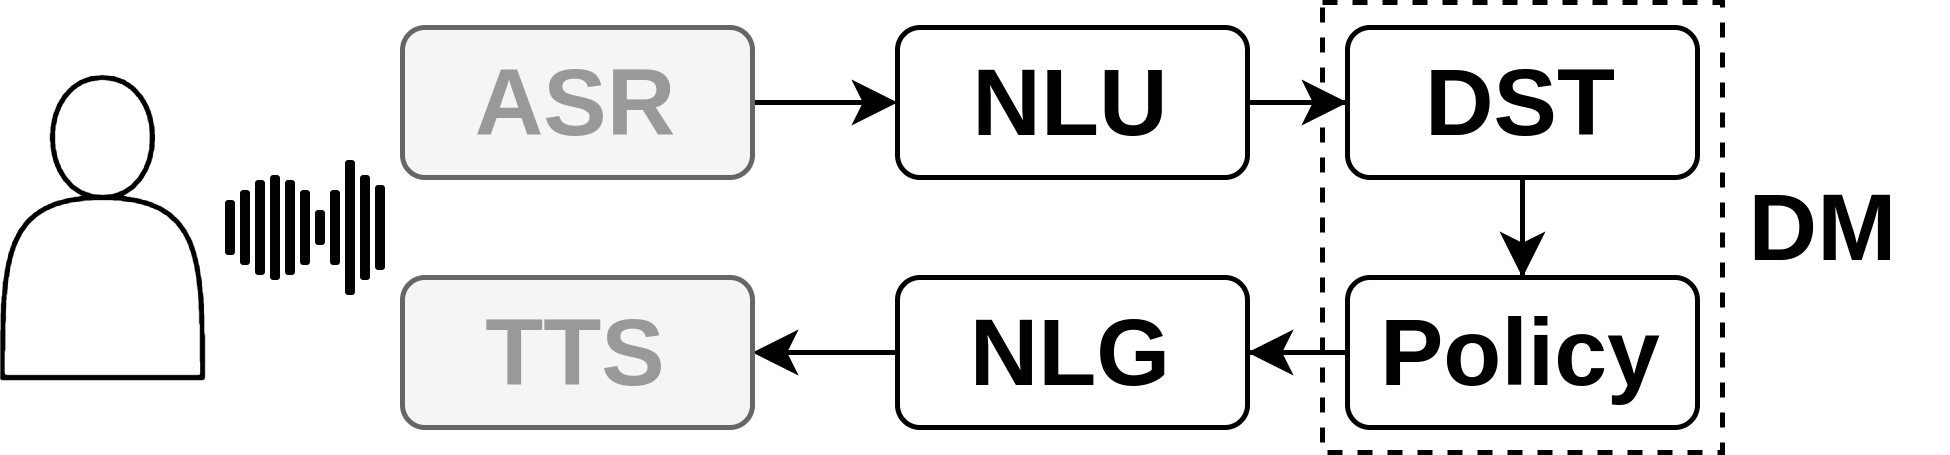
\includegraphics[width=0.80\textwidth]{images/pipeline.png}
    \caption{Overall architecture of task-oriented dialogue system pipeline. The data flow is outlined with arrows. This work does not discuss ASR and TTS modules (depicted in gray) which are often included with the rest of the components.}
    \label{fig:overall}
\end{figure}
A typical approach to task-oriented DS implementation is to create a modular system with several modules that handle the conversation flow together.
An example of such architecture is depicted in Figure \ref{fig:overall}
We shortly discuss the responsibilities of each component:
\begin{itemize}
    \item \textbf{Natural Language Understanding (NLU)} The purpose of NLU is to extract the meaning of input utterances in natural language and transform it into a structured representation, i.e., dialogue acts.
    Basically, the NLU module has three subtasks.
    (1) It has to determine the domain of the utterance, (2) detect the user intent, and (3) capture any slot values, if present.
    \item \textbf{Dialogue State Tracking (DST)} Dialogue state keeps track of the dialogue history, effectively providing the necessary context.
    Dialogue State Trackers are used to update the state with correct values after each turn.
    \item \textbf{Dialogue Policy} The core component of the DS is the dialogue policy.
    Its responsibility is to decide which action the system should take at each turn.
    In other words, Dialogue Policy's responsibility is to guide the dialogue to follow the desired path.
    Dialogue policy and the DST component are sometimes called \emph{Dialogue Manager}.
    \item \textbf{Natural Language Generation (NLG)} When the decision on a system action is made, the system needs to verbalize the action.
    In other words, we need to create an utterance in natural language that expresses the information in the system's underlying representation.
\end{itemize}

The module-based approach is advantageous thanks to its good level of explainability.
In case of low performance, we can track the respective modules' outputs and find the source of problems.
On the other hand, error accumulation makes it difficult to recover from errors made by the modules early on in the pipeline.
Another disadvantage is the way these systems are trained \cite{li-etal-2017-end}
Each component requires specific data annotation.
Thus, obtaining a dataset suitable for training all components can be difficult and costly.
Also, the system design itself is more complicated since it requires the implementation of multiple models.
Because of the aforementioned drawbacks, many current research works focus on dialogue modeling end-to-end, i.e., using systems without explicit components that can be trained jointly.

\subsubsection{Modeling TOD without supervision}
\label{02:no-super}
Here, we introduce some of the challenges concerning TOD modeling in conditions without external structured supervision.
We discuss every step in the pipeline (Section~\ref{02:sec:basics}) separately.

\paragraph{Natural Language Understanding (NLU)}
Recall that the purpose of the NLU component in a traditional dialogue pipeline is to extract the meaning from input utterances in natural language and represent it in a structured way.
Doing this unsupervised is challenging because we do not have the labeled data for training and, moreover, do not know the structure itself in the first place.
However, there are some possible ways to approach this problem.
Works focus on automated annotation schema induction (\ref{sec:relwork-unsup}).
Another way is to let the model handle NLU implicitly, i.e., effectively omitting the NLU step.

\paragraph{Action Selection}
One of the tasks of the dialogue manager is to select the next system action in a given situation.
Most implemented systems implicitly perform this task, i.e., there is no explicit representation of the system action, just a surface realization of it (in the form of verbalized utterance).
The reason for this option is that it requires less supervised labels, which might be hard and costly to obtain.
However, modeling the information about system action can benefit the overall performance~\cite{DBLP:conf/aaai/LiangTCY20}.
We explore the possibility of implicitly learning this information by introducing a network bottleneck in Chapter~\ref{chap:modeling}.

\paragraph{Handling external interfaces}
Task-oriented dialogue systems must provide accurate and complete information based on user requests, which requires interaction with external interfaces such as databases or some structured knowledge base.
To communicate with such external entities, we typically need to design some representation with a predetermined structure so we can construct API queries, etc.
This can be troublesome in a setting where no supervision in the form of labels is present.
Without a known structure, it is very challenging to design the communication protocol with external sources of information.

\subsection{Neural Networks}
\label{background:nns}
The nature of many Natural Language Processing (NLP) tasks is statistical in a way that we can identify patterns seen in data and aim to model the underlying processes.
Therefore, statistical methods in NLP have been extensively used for decades~\cite{manning99foundations}, with varying success.
Although many modeling approaches with various degrees of complexity have been proposed, currently, Neural Network models dominate the field.
Neural architectures are well-known statistical models \cite{GoodBengCour16} that can learn complex data distributions from the presented training data.
Essentially, these models parameterize non-linear functions with millions of parameters learned by optimizing loss objective over the training set using algorithms such as backpropagation~\cite{kelley1960gradient}.

\paragraph{Neural Networks for text processing}
Neural Networks (NN) are widely used across various fields, and NLP is among the most prominent.
However, it is not straightforward how to represent words in NN.
A simple one-hot vector or bag of words representation is insufficient as it throws away a lot of useful information about the relations between words, their position, etc.
Traditional statistical N-gram models \cite{jurafsky2000speech} address some of the issues but again discard some positional information and are inherently limited by context size (N-gram length).
A breakthrough in this field, which allowed for successful NN applications, dates back to the works \citep{mikolov2010recurrent} and \citep{mikolov2013distributed}, which build on the principle of word distributional hypothesis and introduced the concept of \emph{word embeddings}.
Word embeddings are multi-dimensional real vectors that capture important information about each word that occurs in some particular input corpora.
When input to an NN, word embeddings accurately represent the word and arguably capture the meaning.
This principle was later improved by introducing large-scale pretrained neural language models such as ELMo~\cite{peters-etal-2018-deep} and BERT~\cite{devlin2019}, which can create contextualized high-dimensional representations.
We introduce these principles in more detail in Section~\ref{background:plms}

\subsection{Recurrent Neural Networks (RNNs)}
\label{background:rnns}
Recurrent Neural Networks are a type of neural network that is well-suited for processing sequential data\cite{GoodBengCour16}. Sequential data is ordered in time, such as text or audio.
RNNs can learn long-range dependencies between different parts of the input sequence, which makes them well-suited for tasks such as machine translation, text summarization, and question answering.
The motivation for RNNs comes from human language being sequential by nature; therefore, sequential dependencies must be handled.

The characteristic feature of an RNN is a recurrent connection incorporated into the architecture.
This means that the network's output at a given time step is fed back into the network at the next step. This allows the network to encode some information and pass it for future processing, effectively allowing for a concept of memory.

Basic RNN consists of 3 weight matrices: $W_{i}$ to process the input, $W_h$ to process the hidden state, and $W_o$ to construct output.
The computation of output sequence $\mathbf{y} = \{y_0, ..., y_n\}$ from an input sequence $\mathbf{x} = \{x_0, ..., x_n\}$ proceeds in the following steps:
\begin{enumerate}
    \item An initial hidden state $h_0$ is constructed
    \item For time step $t$, first hidden state $h_t$ is obtained using the formula $h_t = f(W_hh_{t-1} + W_ix_t)$. Then, the output is computed as $y_t = W_oh_t$
\end{enumerate}
Note that the output sequence has the same length as the input sequence, which is useful for sequence tagging problems.
However, RNNs can also be used for sequence classification, in which case only the last hidden state is considered, or the encoder-decoder setup can be used in which one network is used to encode the sequence and the second one is used to generate the output which can therefore be of different length.

\paragraph{RNN cell improvements}
Vanilla RNNs are difficult to train and often fail to memorize long-term dependencies correctly.
Therefore, several extensions were proposed such as LSTM \cite{hochreiter1997} or GRU \cite{cho-etal-2014-properties}
These more complex types of RNNs can learn long-range dependencies more effectively.
LSTM and GRU cells have several gates that control how information flows through the cell.
These gates allow the RNN cell to learn how to forget irrelevant information and remember important parts of the input.
NLP models often employ \emph{bidirectional} RNNs to improve modeling capabilities further, allowing for processing both left and right context.

\paragraph{Training RNNs}
RNNs are trained using a technique called Backpropagation Through Time \cite{werbos1990backpropagation}.
Backpropagation Through Time is a method for training neural networks that deal with sequential data.
The basic idea is to break the sequence into a number of time steps and then train the network on each time step individually.

\paragraph{Encoder-Decoder RNNs with attention}
The encoder-decoder RNN is useful for text-generation tasks like summarization or machine translation.
However, it is very difficult to train RNN on longer sequences.
Therefore, improvements were proposed \cite{bahdanau2014neural,luong-etal-2015-effective} that allow the decoder network to attend to the input sequence and bypass the need to memorize all the information in the hidden state.

\subsection{Transformer}
\label{background:trafo}
\begin{figure}[ht]
    \centering
    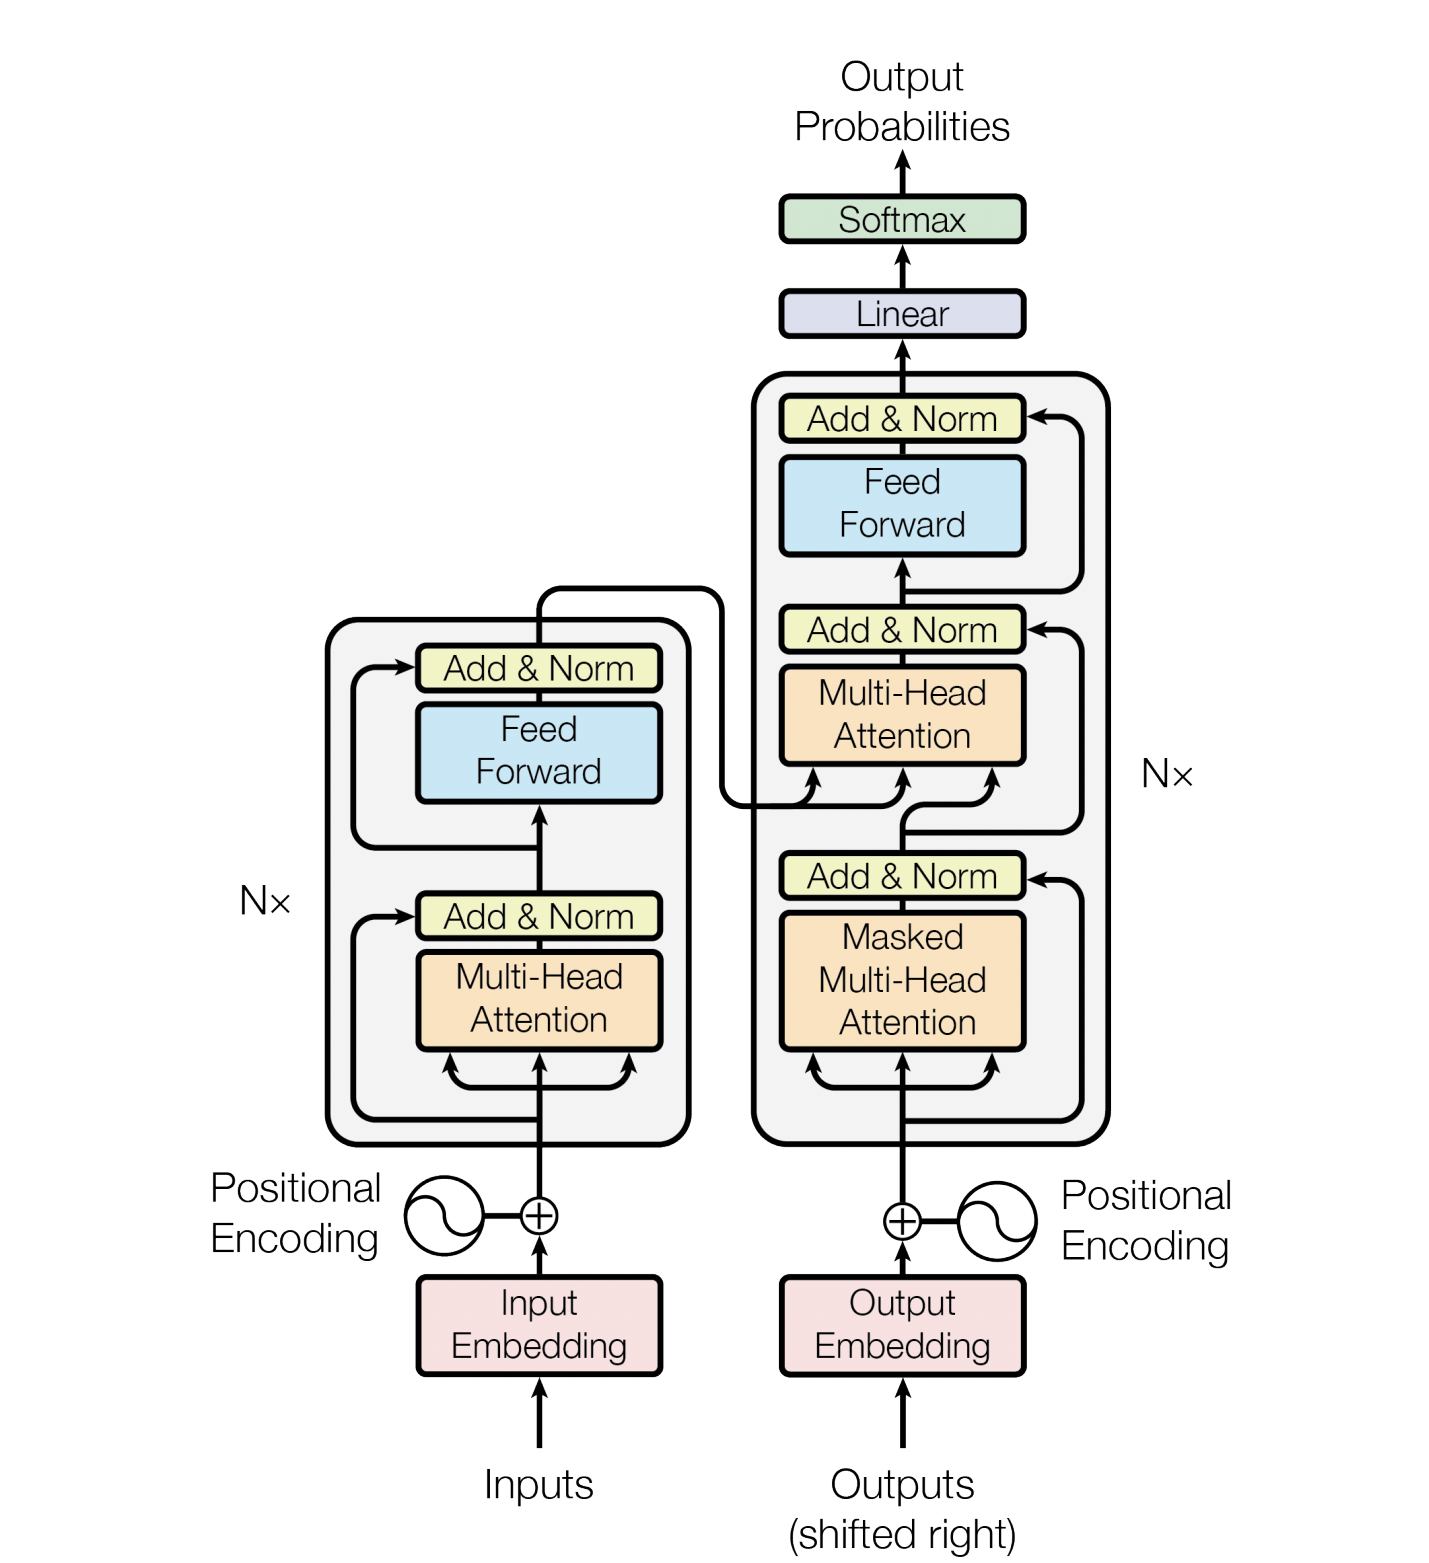
\includegraphics[width=0.9\textwidth]{images/transfo-arch.png}
    \caption{The Transformer architecture as proposed by \citep{vaswani2017attention}. We can see the encoder (left) and decoder (right) stacks and their interconnection.}
    \label{fig:trafo}
\end{figure}
The Transformer architecture is another neural network architecture capable of processing sequential data.
It was first proposed in \citet{vaswani2017attention}.
Unlike RNNs, the Transformer architecture does not work with a hidden state that is being passed forward in time.
Instead, the architecture is based solely on the attention mechanism, which allows the model to learn long-range dependencies between different parts of the input sequence.
The high-level equation describing the self-attention mechanism is formulated as follows:
\begin{equation*}
    Att(Q,K,V) = softmax(\frac{QK^T}{\sqrt{d_k}}V)
\end{equation*}
where $Q$, $K$ and $V$ are trainable square weight matrices corresponding to \emph{queries}, \emph{keys} and \emph{values} and with dimension $d_q$, $d_k$, $d_v$ respectively.
The attention mechanism allows the model to focus on different parts of the input sequence when producing the output sequence.
For example, if the model is translating a sentence from English to German, the attention mechanism can allow the model to focus on the English words most relevant to the German words that need to be produced.

The original Transformer architecture comprises an encoder and a decoder, depicted in Figure~\ref{fig:trafo}.
The encoder takes the input sequence and produces a sequence of hidden representations.
The decoder then takes these hidden representations and produces the output sequence.
The attention mechanism is used at both the encoder and decoder to allow the model to use different parts of the input sequence when producing the output sequence.
Depending on the use case, the decoding process might be performed both as autoregressive or non-autoregressive.

Both the encoder and decoder are basically a stack of self-attention layers.
Each self-attention layer takes the hidden representations from the previous layer and produces a new set of hidden representations.

The decoder also includes an attention component that allows the model to attend to the output sequence generated so far when producing the next token.
This allows the model to learn how to generate the output sequence consistently with the input sequence and the prefix generated so far.

The Transformer architecture has been shown to achieve state-of-the-art results on various natural language processing tasks. 
Moreover, the Transformer architecture was used as a base for many models pre-trained on large natural language corpora, allowing efficient transfer of the learned information to downstream tasks and thus revolutionizing the NLP field.

\section{Pretrained Language Models (PLMs)}
\label{background:plms}
The appearance of PLMs marked a new era in NLP.
Although Language Modeling with neural networks has been in the community focus for some time with transforming works such as  \citet{mikolov2010recurrent,mikolov2013distributed}, it was not until RNN-based models such as ELMo \cite{peters-etal-2018-deep} and ULMFiT \cite{howard-ruder-2018-universal} were proposed that we were able to create PLMs that could be finetuned for a variety of tasks with comparably low data requirements.

Shortly after ELMo, models based on the Transformer architecture started to appear, such as BERT for efficient language encoding \cite{devlin2019} or GPT for generation \cite{radford2018improving}.
BERT introduced a novel approach to Transformer usage by employing only the encoder part of the original Transformer architecture.
Importantly, BERT pretraining introduced the task of Masked Language Modeling, randomly masking some of the input tokens and reconstructing them correctly at the output.
Additionally, BERT is trained to estimate the probability that two input sentences follow each other.
These pretraining techniques make BERT great at encoding natural language inputs into useful representations.
GPT, on the other hand, consists only of Transformer decoder blocks.
It is trained for next token prediction and can perform autoregressive Language Modeling.
Therefore, GPT is a perfect candidate for a base model to be finetuned on language generation tasks, including data-to-text, summarization, etc.


Both BERT and GPT showed great potential for finetuning downstream tasks and established themselves as strong baselines for many NLP tasks and benchmarks.
They are often referred to as \emph{foundational} models because of their language understanding and generation abilities and the potential to apply these abilities to various tasks.
From a certain point of view, the usability of PLMs lies in the ability to create useful and contextual representations of input words and phrases, often called \emph{(word) embeddings}.
This ability has been observed in the word2vec model \cite{mikolov2013distributed} and improved by ELMo~\cite{peters-etal-2018-deep}, BERT~\cite{devlin2019}, SBERT~\cite{reimers2019sentence} and others.

Many model architectures based on Transformer blocks followed both for encoders \cite{liu2019roberta,reimers2019sentence}; decoders \cite{radford2019language,brown2020language} or even sequence-to-sequence \cite{raffel2020exploring,lewis-etal-2020-bart}.
The NLP community largely adopted these models.


\subsection{Large Language Models (LLMs)}
The foundational models changed the NLP paradigm but still need substantial in-domain data to perform some tasks well.
Moreover, finetuning those larger models requires more computational resources.
Therefore, more lightweight methods were proposed to adapt the models to downstream tasks, such as Transformer Adapters \cite{pfeiffer2020AdapterHub}.
However, as researchers started to scale up the models with GPT-2 and GPT-3 leading the efforts \cite{radford2019language,brown2020language}, new abilities emerged \cite{wei2022emergent}.
With model sizes exceeding billions of parameters, the large pre-trained Transformer decoders can perform many tasks that they were not explicitly trained for \cite{brown2020language}.
Such large models can perform tasks like summarization, translation, question answering, or even reasoning and arithmetics to some extent without any task-specific training.
However, it is unclear how many examples of the abovementioned tasks were seen during these models' training phase.
Those tasks can be presented to the LLMs purely in the form of textual task descriptions in the inference time.
This approach of \emph{in-context learning} is frequently used with great success \cite{min2022rethinking,dong2022survey}.
The textual input for LLMs is frequently called a \emph{prompt}.

\paragraph{On LM scaling}
Scaling laws in language models describe the relationship between the size of a language model and its performance.
It has been shown that with the next token prediction objective (which is what virtually all LMs are trained for), some abilities start to emerge when exceeding a certain size threshold \cite{kaplan2020scaling}.
However, bigger models also need to be trained longer and with more data \cite{hoffmann2022training}
In general, larger language models tend to perform better than smaller models but also require more computational resources to train.
This line of research can help us understand how the size of a language model affects its performance and predict the performance of a language model before it is trained.

\paragraph{Instruction Tuning}
Although the LLMs have great abilities and potential to accomplish various tasks, providing them with correct instructions is not always straightforward.
Therefore, significant effort was made to \emph{align} the LLMs better with the human requirements.
Consequently, even rather inexperienced users can instruct the model to accomplish custom tasks according to their needs.
For this purpose, reinforcement learning techniques were explored \cite{ziegler2019fine,ouyang2022training}.
Although these techniques proved to be quite effective, the process is still very demanding in collecting user feedback.
Consequently, several datasets were proposed \cite{supernaturalinstructions,black2022gpt} that contain tasks like summarization, reasoning, etc. formulated using instructions in natural language and desired outputs.
These datasets allow tuning of the models using reinforcement learning or supervised finetuning methods.

\paragraph{Prompt engineering vs. LLM finetuning}
The in-context learning approach has great advantages because it makes it possible to obtain great performance from LLMs by simply formulating the task and desired output structure in the LLM input (i.e. prompt).
Although this approach might be very efficient for some tasks, especially those that are well described in the corpora available to the LLM during training \cite{wei2022emergent}, some more specific tasks might yield better results after finetuning of the model \cite{tu-etal-2022-prompt}.
However, the LLM finetuning process is quite demanding in terms of computational resources.
Therefore, alternative approaches were proposed, such as LoRA \cite{hu2021lora} or Transformer Adapters \cite{pfeiffer2020AdapterHub}.
These approaches make LLM finetuning much more accessible.
In general, both finetuning and in-context learning can offer great performance and be beneficial in certain situations~\cite{mosbach-etal-2023-shot}.

\section{Variational autoencoders}
\label{02:sec:vae}
\begin{figure}[t]
    \centering
    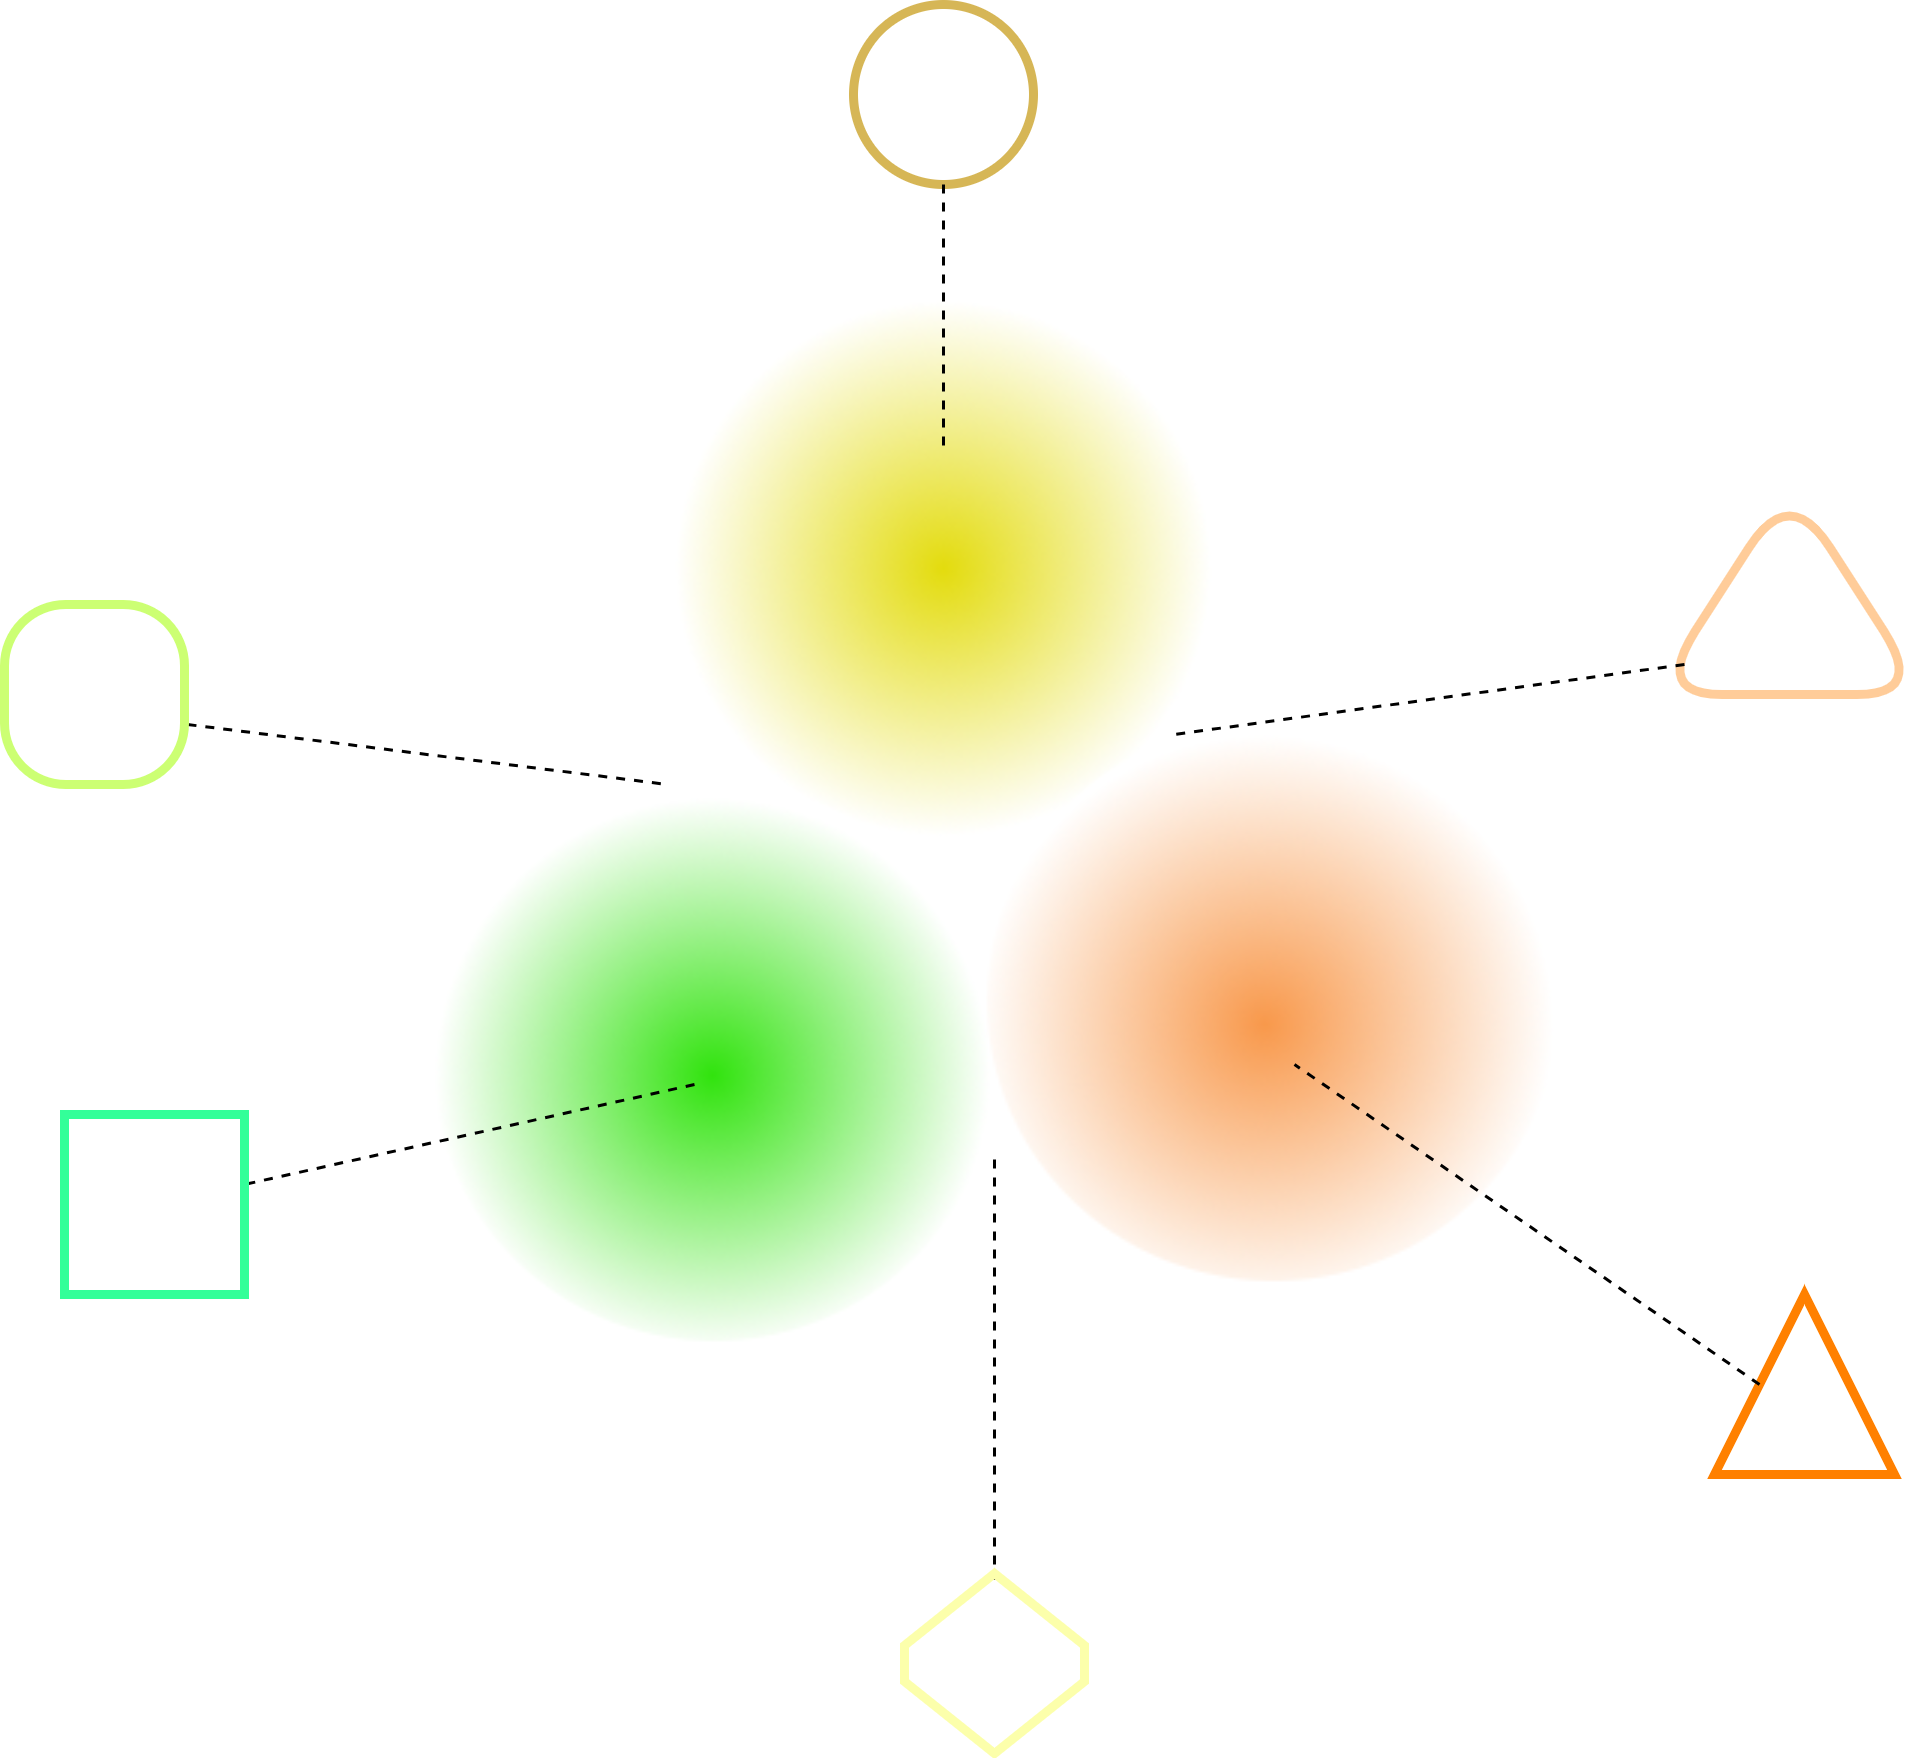
\includegraphics[width=0.46\textwidth]{images/VAE.png}
    \caption{Variational autoencoder latent space. Colors and different classes by shapes distinguish the encoder distributions. It can be seen the interpolation between two sampled points is meaningful}
    \label{fig:vae}
\end{figure}
\begin{figure}[t]
    \centering
    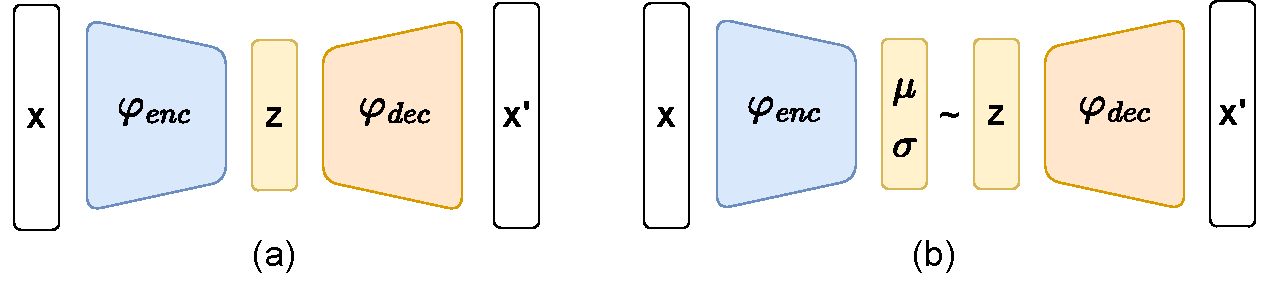
\includegraphics[width=0.9\textwidth]{images/enc-dec.pdf}
    \caption{Illustration of differences between the architectures of a vanilla autoencoder (a) and its variational version (b). The VAE encodes the input by predicting parameters of probabilistic distribution from which the data are drawn rather than encoding the data directly into a hidden representation, as done with the vanilla autoencoder.}
    \label{fig:vae-vs-ae}
\end{figure}
In neural network training, the network learns to create internal data representations to accomplish a given task.
In the case of autoencoders, the task is to encode an input $\mathbf{x}$ in a way that allows for its reconstruction into the original form.
The autoencoder model consists of an encoder function $\varphi^{enc}$, which encodes an input $\mathbf{x}$ into a latent representation $\mathbf{z}$, and a decoder $\varphi^{dec}$, which models the conditional re-generation probability $p(\mathbf{x}|\mathbf{z})$.
In the case of sequence autoencoders, both the encoder and decoder can be realized with an RNN.
However, vanilla autoencoders often fail to extract global semantic features of natural language sequences \cite{bowman2015generating}; therefore, adjustments must be made to obtain better representations.
The technique proposed by \citet{kingma2013auto} uses the Variational Autoencoder (VAE) framework to tackle this issue.
The architecture is modified so that $\varphi^{enc}$ represents a recognition model $q(\mathbf{z}|\mathbf{x})$ which parameterizes an approximate posterior distribution over $\mathbf{z}$.
Figure~\ref{fig:vae-vs-ae} illustrates the differences.
VAEs impose prior distribution on the latent variable $\mathbf{z}$, which acts as regularization during training and makes drawing samples from $q$ possible.
Consequently, the VAE latent space is smooth because it is possible to interpolate between two points and obtain reasonable representations.
The latent space structure is depicted schematically in Figure \ref{fig:vae}.
The modeled distributions are typically Gaussian; the prior is the standard normal distribution $N(0, 1)$ in that case.

We can realize the encoder and decoder modules in VAE using neural networks.
However, there is a drawback regarding the implementation of sampling.
The sampling operation is not differentiable and, therefore, cannot be trained using standard approaches.
A solution to this problem is to use the \textit{reparameterization trick} \cite{kingma2013auto}.
The reparameterization trick exploits the fact that a random variable under a certain conditional distribution can be expressed as a deterministic transformation of some other variable with an independent marginal distribution.
Distributions that allow us to do such a transformation include \textit{Gaussian, Logistic} or \textit{Gumbel}~\cite{jang2016categorical}.

\subsubsection{VAE latent space discretization}
\label{02:sec:vae_discrete}
Although VAE training yields robust representations that are also more interpretable thanks to the regularized latent space, in some cases, we require the latent representations to be discrete.
The motivation is mainly to improve interpretability and uncover underlying processes in sequential tasks.
Incorporating discrete variables into neural network models is problematic because the widely used backpropagation algorithm requires smooth differentiable functions to propagate the gradients correctly.
\cite{van2017neural} propose a vector quantization technique to discretize the latent variables in VAEs.
Another approach is to use the Gumbel-softmax distribution \cite{jang2016categorical} that, together with the reparameterization trick (Section \ref{02:sec:vae}), enables work with categorical variables while not breaking the gradient flow in the network.

\subsection{Variational Recurrent Neural Networks}
\label{02:sec:vrnn}
\begin{figure}
    \centering
    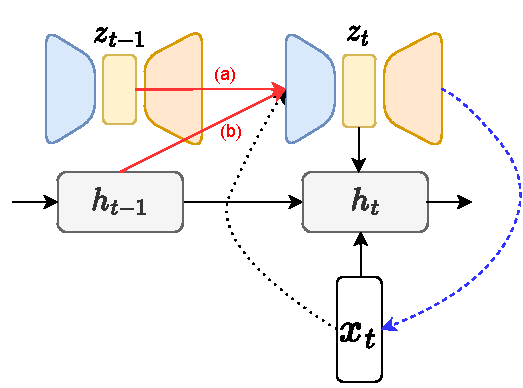
\includegraphics{images/DVRNN.pdf}
    \caption{A schematic architecture of the VRNN model. The input in time step $t$ is used as input to the variational autoencoder (black dotted line). The VAE prior is conditioned either on the previous hidden state (a) or previous latent variable $z_{t-1}$ (b) (red lines). To regenerate the output, the decoder from latent space is used (blue dashed line). Finally, the hidden state update is based on latent representation $z_t$, previous hidden state, and current input (solid black lines).}
    \label{fig:DVRNN}
\end{figure}
The VRNN model \cite{chung2015recurrent} exploits the idea of variational training to model sequences with latent states.
Intuitively, the VRNN model can be seen as a recurrent network with a VAE in every timestep.
The VRNN architecture is depicted in Figure~\ref{fig:DVRNN}.
It assumes that the sequence of observations was generated from a sequence of unknown latent states and uses a VAE to model these latent variables $\mathbf{z}$.
Formally, we want to estimate the joint probability distribution of a sequence of observations and corresponding latent variables $p(\mathbf{x}, \mathbf{z}) = p(\mathbf{x}|\mathbf{z})p(\mathbf{z})$.
The conditional distribution $p(\mathbf{x}|\mathbf{z})$ is parameterized with a neural network.
However, we still need to estimate the posterior $p(\mathbf{z}|\mathbf{x})$ to connect the latent variables with the observations.
The VAE uses a variational approximation $q(\mathbf{z}|\mathbf{x})$ that allows maximizing the evidence lower bound (ELBo) of the log-likelihood of the data:
\begin{equation}
\begin{split}
    \log~p(\mathbf{x}) \ge -\mathrm{KL}(q(\mathbf{z}|\mathbf{x})||p(\mathbf{z}))\\ + \mathbb{E}_{q(\mathbf{z}|\mathbf{x})}[\log~p(\mathbf{x}|\mathbf{z})]
    \label{eq:vae}
\end{split}
\end{equation}
where KL is the Kullback-Leibler divergence.

We consider a prior network $\varphi_{prior}$ and a posterior network $\varphi_{post}$, which compute the parameters of $p(\mathbf{z})$ and $q(\mathbf{z}|\mathbf{x})$ respectively.
In a VRNN, $\varphi_{prior}$ and $\varphi_{post}$ additionally depend on the RNN hidden state $\mathbf{h}^t$ to allow for a context-aware prior distribution.
In each time step, we obtain the distribution parameters as follows:
\begin{equation}
\label{eq:distr_theta}
\begin{gathered}
    \mathbf{\theta}_{q}~=~\varphi_{post}(\mathbf{h}^t, \varphi_{enc}(\mathbf{x}^t))\\
    \mathbf{\theta}_{p}~=~\varphi_{prior}(\mathbf{h}^t)
\end{gathered}
\end{equation}
where $\varphi_{enc}$ is the encoder and $\theta_q, \theta_p$ are parameters of the respective distributions.
With distribution parameters available, we can sample the latent variable and predict the output:
\begin{equation}
\label{eq:x_infer}
\begin{gathered}
    \mathbf{z}^t~\mathtt{\sim}~p(\mathbf{z};\theta_{p})\\
    \mathbf{x}^t~=~ \varphi_{dec}(\mathbf{z}^t)
\end{gathered}
\end{equation}
where $\varphi_{dec}$ represents the decoder network.
The update of the hidden state $\mathbf{h}^t$ is as follows:
\begin{equation}
    \label{eq:hidden_update}
    \begin{gathered}
        \mathbf{h}^{t+1} = \text{RNN}([\varphi_{enc}(\mathbf{x}^t),\varphi_{z}(\mathbf{z}^t)], \mathbf{h}^t)
    \end{gathered}
\end{equation}
where $[.,.]$ is concatenation, $\varphi_z(.)$ is a feature extractor, and $\text{RNN}()$ is a step transition function of a recurrent neural network, in our case an LSTM \cite{hochreiter1997}.

\subsection{Latent Action Spaces via Variational Auto-encoding - LAVA}
\label{02:sec:lava}
\todo{More details}
The LAVA framework~\cite{lubis-etal-2020-lava} focuses on learning latent variables in a way that they store dialogue-related actions.
To achieve this, they employ VAE-based model architecture.
The architecture comprises an RNN utterance encoder, VAE module, and RNN decoder.
They train the model in multiple stages and different variants.
Specifically, they first pretrain the encoder module using an autoencoding objective.
Then, they use the pretrained decoder and train an additional encoding module for the next response prediction.
In the end, they use reinforcement learning to tune the model parameters further.
Formally, the authors first train an encoder-decoder network with an autoencoding objective version of ELBo parameterized by $\phi$.
\begin{equation}
    \mathbb{L}_{ae}(\phi) = \mathbb{E}_{q_{\phi}(\mathbf{z}|\mathbf{x})}[\log~p_{\phi}(\mathbf{x}|\mathbf{z})] -\mathrm{KL}(q_{\phi}(\mathbf{z}|\mathbf{x})||p(\mathbf{z}))
\end{equation}
where $\mathbf{x}$ represents dialogue utterance.
Then, they train the response generation network parameterized by $\theta$ using the lite ELBo objective~\cite{lubis-etal-2020-lava}.
\begin{equation}
    \mathbb{L}_{lite}(\theta) = \mathbb{E}_{q_{\theta}(\mathbf{z}|\mathbf{c})}[\log~p_{\theta}(\mathbf{x}|\mathbf{z})] - \beta\mathrm{KL}(q_{\theta}(\mathbf{z}|\mathbf{c})||p(\mathbf{z}))
\end{equation}
where $\mathbf{c}$ is a sequence of utterances representing the dialogue context.
For the second step, the decoder network $p_{\theta}$ is initialized by pretrained $p_{\phi}$.

\section{Memory Networks}
\label{02:sec:mem_nn}
\begin{figure}[t]
    \centering
    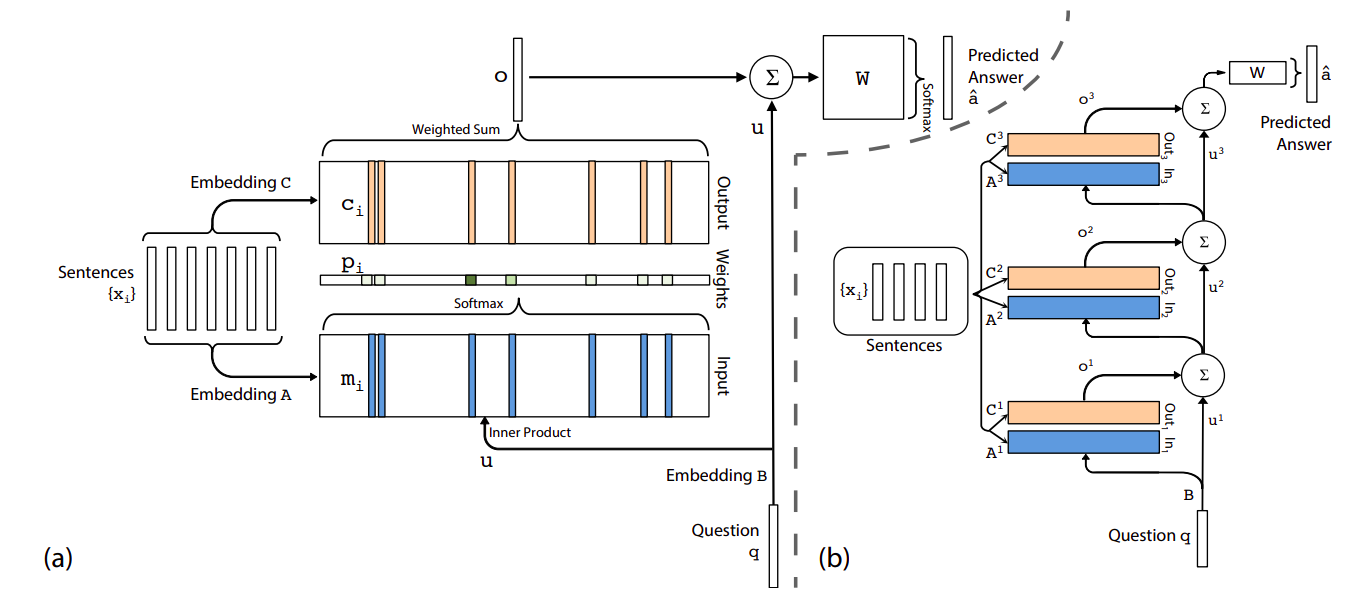
\includegraphics[width=\textwidth]{images/e2e_mem_nn.png}
    \caption{The end-to-end Memory Network model introduced in \citet{sukhbaatar2015end}. It shows the computation process of (a) a single-layer and (b) a 3-layer model version. }
    \label{fig:e2e_memnn}
\end{figure}
The Memory Network model (MemNN) addresses the issue associated with RNN networks, which typically suffer from catastrophic forgetting and exponential decay of stored information \cite{neil2016phased}.
The Memory Network model was originally introduced in \citet{DBLP:journals/corr/WestonCB14}.
\subsection{The Memory Network architecture}
The key idea behind memory networks is to incorporate an external memory component into the network architecture, allowing the model to store and access information over long sequences of inputs.
The memory component acts as a separate storage module, similar to a computer's memory, which the network can read from and write to during its computation.
The MN model architecture's main component is a memory array $\mathbf{m} = \{\mathbf{m}_1,...,\mathbf{m}_n\}$.
The basic Memory Network takes an input $\mathbf{x}$ and processes it in four processing steps:
\begin{enumerate}
    \item The input $x$ is processed with \emph{input feature map} $I$ to obtain internal representations of the input $I(x)$.
    \item The memory array is updated using the \emph{generalization component} $G$. In this step, each memory entry gets updated following the equation $\mathbf{m}_i = G(\mathbf{m}_i, I(\mathbf{x}), \mathbf{m})$.
    \item The output features are computed with the \emph{output feature map} using the memory and transformed input $ o = O(I(\mathbf{x}, \mathbf{m})$
    \item Finally, the output representation is used to decode the final response: $r = R(o)$
\end{enumerate}

The components $I, G, O$, and $R$ can be represented with any function capable of doing the task.
However, in most cases in the literature, we see models that use neural networks to instantiate these components.
Consequently, the whole model is end-to-end differentiable and thus trainable with algorithms such as backpropagation.
We talk about Memory Neural Networks (MemNNs).
Although various kinds of data can be input and output to MemNNs in general, we consider only MemNNs that work with text in this work.
Let us describe a basic MemNN for text.
When given text input, such a basic model can save each text memory into a new memory slot.
Therefore, old memories are not updated, and new inputs are stored sequentially.
The most interesting components of this simple text model are $O$ and $R$.
The $O$ module scores the saved memory vectors given text input $x$ and subsequently retrieves $k$ supporting entries with the highest scores from the memory.
To produce a response, the $R$ module takes the input $x$ and $k$ retrieved memories and generates an output either by copying one of the memories or truly generating new outputs, for example, with an auto-regressive RNN decoder. 

\subsection{Multi-hop end-to-end MemNN}
The MemNN architecture's disadvantage is that it requires supervision at each layer during training, as pointed out by \citet{sukhbaatar2015end}.
In this work, the authors address this problem and present a fully end-to-end trainable memory network model, which we call \emph{e2eMemNN}.
In the e2e MemNN, we input a set of vectors $x$ to be stored in the memory and a query $q$.
Each input $x_i$ is then embedded with two distinct embedding functions $E_m$ and $E_c$ to obtain a memory entry $m_i$ and corresponding output embedding $c_i$, respectively.
The query $q$ is then embedded as well with the different function $E_q$ to obtain query embedding $u$.

\begin{figure}[t]
    \centering
    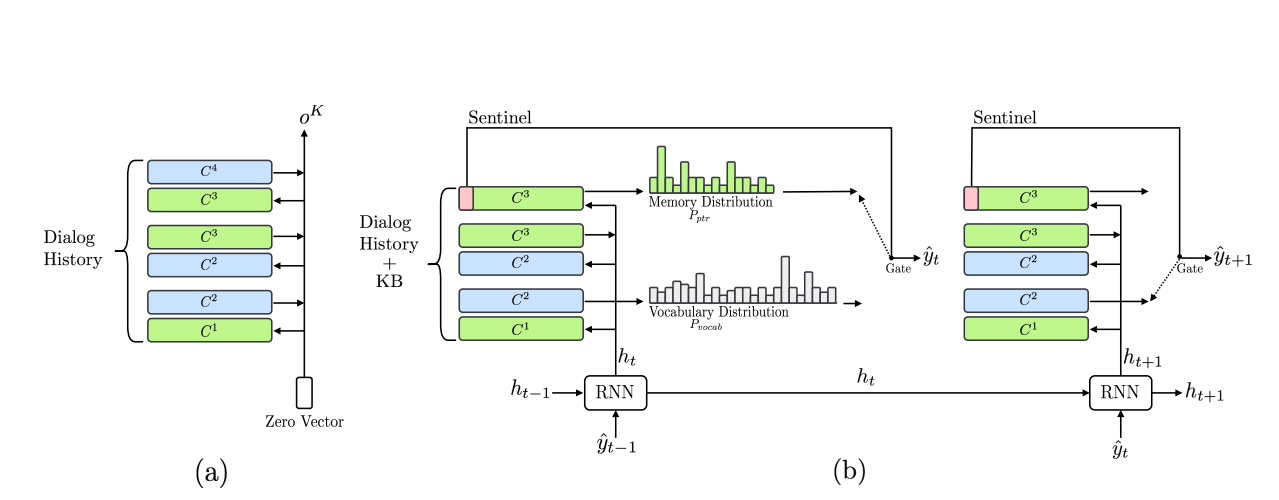
\includegraphics[width=\textwidth]{images/mem2seq.png}
    \caption{The Mem2Seq model \cite{madotto-etal-2018-mem2seq} showing the memory encoder with 3 hops (a) and 2 steps of the memory decoder (b) }
    \label{fig:mem2seq}
\end{figure}

Upon embedding the inputs, a memory distribution $p$ is computed as a match between $u$ and each memory $m_i$ as $softmax (u^Tm_i)$.
The memory distribution $p$ is then used to create an output $o$ computed as a weighted sum over the output embeddings $\sum_i p_ic_i$.
The output $o$ is then used to produce the final answer, which can be a categorical label or textual response generated with an auto-regressive model.

The authors also introduce a multi-layer version of this model.
In the multi-layer version, each layer $k$ has distinct embedding matrices $E^k_m$ and $E^k_c$. The output $o_k$ from layer $k$ is used to form input query embedding $u_{k+1}$ to the layer $k+1$: $u_{k+1} = u_k + o_k$.
The multi-layer processing is sometimes referred to as \emph{multi-hop} where a \emph{hop} refers to processing by one layer.

\subsection{Mem2Seq model}
\label{02:sec:mem2seq}
The Mem2Seq model \cite{madotto-etal-2018-mem2seq} is a task-oriented dialogue model that builds on top of the end-to-end architecture introduced in \citet{sukhbaatar2015end}.
The architecture is described in Figure \ref{fig:mem2seq}.
The model consists of encoder and decoder parts.
The encoder is a 3-hop memory network that encodes the dialogue context.
The more interesting part is the decoder, a recurrent neural network enhanced with a memory network in every time step.
This memory network contains conversation history and knowledge base entries encoded as memory vectors.
At each step, the hidden state of the RNN is used as a query vector. Then, a distribution over memory is computed, as described earlier. 
Also, a distribution over vocabulary is computed from the RNN hidden state, similar to standard RNN-based decoders.
One special entry is added to the memory, so-called \emph{sentinel}.
The vocabulary distribution generates the next token if the highest probability is assigned to the sentinel token.
Otherwise, the next token is chosen according to the memory distribution.
In other words, the model uses the RNN state at each generation step to decide whether to copy something from memory (conversation history + knowledge base info) or generate an arbitrary new token from vocabulary distribution.
This way, the model can use information from the past effectively.

\section{Datasets}
\label{02:sec:input-data-desc}
We describe some of the most prominent datasets we use for our experiments.
Most of them are largely used in the dialogue community and provide common benchmarks used for the evaluation.
All these datasets have several task-oriented dialogue properties in common that define the conversation according to \cite{young_pomdp-based_2013}:
\begin{enumerate}
\item \textbf{Domain(s)} define the topic (or range of topics) which are mentioned in the dialogue. There can be several domains per dialogue.
\item \textbf{Task} -- the users in each dialogue are attempting to reach a certain goal (such as booking a restaurant or finding a tourist attraction).
\item \textbf{Turns} We consider \emph{turn-taking} dialogues, i.e.\ the participating sides exchange utterances alternately.
One such utterance exchange is called a dialogue turn.
Utterance is considered the linguistic realization of the speaker's thoughts and will. It can be spoken or written. 

The meaning of each utterance can be represented in a structured way with \textbf{Dialog Act(s)} \cite{Weisser2016}.
It is a meta-information that emerges from the respective utterance and qualifies it. It describes the beliefs, desires, and intentions.
Dialogue acts can be represented using \emph{Domains}, \emph{Intents}, and \emph{Slots} as described in Section~\ref{02:ds-background}.
The slots can also be further categorized.
Typically, we define \emph{inform} and \emph{request} slots (Table~\ref{02:tab:inf-req}). Inform slots correspond to information provided by the user and inform about constraints the user has, while request slots communicate the kind of information that the user wants to obtain.
\begin{table}[tp]
    \centering
    \begin{tabular}{l|l}
    \toprule
         \textbf{User} & \texttt{I am looking for a {\color{cyan!80!yellow!80!black!100 }chinese} restaurant} \\
         \textbf{System} & \texttt{The Golden Dragon is a nice place in the South} \\
         \textbf{User} & \texttt{Please, give me their {\color{orange!50!yellow!90!black!100!}phone number} and {\color{orange!50!yellow!90!black!100!}address}} \\
         \bottomrule
    \end{tabular}
    \caption{An illustration of the difference between {\color{cyan!80!yellow!80!black!100 }\textbf{inform}} and {\color{orange!50!yellow!90!black!100!}\textbf{request}} slots.}
    \label{02:tab:inf-req}
\end{table}
The intent represents the user intention, i.e., the sub-goal that the user wants to achieve with a particular utterance.
For an example of dialogue act annotation, we refer to Figure~\ref{fig:das} in Section~\ref{02:ds-background}.
Slots represent the attributes that instantiate the dialogue act.
Each domain is associated with certain intents; each intent can be combined with multiple slots. A slot, however, can be used by multiple intents as well.
We provide statistics about the dialogue datasets we use in this work in Table \ref{02:tab:data_stats} and some samples in Tables \ref{02:tab:mw_example} and \ref{02:tab:smd_example}.
\end{enumerate} 

\subsection{Datasets description}
\label{02:sec:data-desc}
\paragraph{MultiWOZ} (\textbf{MW}) is an established task-oriented dataset introduced by \cite{budzianowski-etal-2018-multiwoz}.
It has been released in several versions; the standard most commonly used nowadays are MultiWOZ 2.1 and MultiWOZ 2.2.
MultiWOZ 2.2 is an improved version of the original dataset by (1) fixing some annotation errors, inconsistencies, and ontology issues and (2) adding slot span annotations for utterances.
MultiWOZ contains over 10,000 annotated dialogues and spans multiple domains - restaurant and hotel reservations, tourist attraction search, taxi and train reservations.
While some of the dialogues use only a single domain, most of them are multi-domain.
For example, after finding a restaurant, the user also asks for a hotel to stay at and orders a taxi.
This makes the dataset more relevant to real-world use cases.

The data were gathered via a crowd-sourcing Wizard-of-Oz scheme described in \cite{wen-etal-2017-wizard-of-oz}.
As MW is used most in our work, we provide further information on the data distribution in Figure~\ref{02:fig:mw-dist} and a sample of the data in Table~\ref{02:tab:mw_example}.

\paragraph{DSTC2} \cite{henderson_robust_2014} was introduced as a part of a challenge to improve state tracking within dialogue systems. It contains over 3,000 dialogues covering a single domain around restaurant reservations. The dialogue corpus was collected using Amazon Mechanical Turk with a POMDP-based spoken dialogue system. It is the only human-machine dataset in our collection.

\paragraph{CamRest676} (\textbf{CR}) \cite{wen2016network} is another crowd-sourced dialogue corpus gathered via the Wizard-of-Oz scheme. CamRest, with its 676 conversations, is the smallest of the datasets used in this work, and it is also a single-domain dataset focused on helping users to find a restaurant in Cambridge, UK. 

\paragraph{Schema-guided dialogue} (\textbf{SGD}) is a large (more than 20,000 dialogues) multi-domain (around 20 domains covered) dataset containing in total 45 API services based on a pre-defined schema. First, the data was collected via a simulator that interacts with the API services, and then the dialogues were paraphrased using crowd-sourcing. \\

\paragraph{ATIS} (\textbf{AT}) \cite{hemphill_atis_1990} contains utterances taken from conversations about flight searches and reservations. \footnote{There are multiple ATIS data versions available. We used one from \url{https://www.kaggle.com/siddhadev/atis-dataset-from-ms-cntk}.}

\paragraph{Cambridge SLU} (CS) \cite{henderson2012discriminative} resembles the CamRest 676 dataset but is larger and focuses only on other user parts of the conversations.
Therefore, Cambridge SLU is not a true dialogue dataset as it contains only single utterances and can be used solely for the NLU task.

\paragraph{Stanford Multidomain Dialogues} (\textbf{SMD}) \cite{eric-etal-2017-key} contains concise dialogues between a driver and an in-car virtual assistant about appointments, navigation, and weather.
The dataset assumes interaction with the database or external APIs.
However, the information is provided with each dialogue in the form of relevant Knowledge Base entries.
We provide an example from the data in Table~\ref{02:tab:smd_example}.

\subsection{Dataset limitations}
\label{02:sec:data-limits}
Although the number of dialogue datasets is quite big, and there is arguably a lot of variance with respect to the size, data collection approach, etc. there are some limitations that are inherently present with this type of data.
We want the data to be used for two main purposes: training and evaluation.
Both these aspects are influenced by the static nature of the data.
Dialogue is a dynamic process that requires interaction.
Hundreds of alternatives exist for a specific conversation that represents a certain information exchange with different phrasing, length, or turn ordering.
All of this is impossible to capture in a static dataset.
Therefore, dialogue modeling should somehow take this into consideration.
A similar issue stems from the fact that there are multiple valid responses under a specific dialogue context, not only with respect to the phrasing but also considering dialogue acts.
Consequently, model evaluation with these data tends to penalize generated responses that are meaningful and relevant but do not correspond to the ground truth found in the data.

Another consideration regards the focus of these datasets.
We almost exclusively work with \emph{task oriented} datasets in this work.
Therefore, the instances contain some structured annotation, most frequently in a dialogue state.
While this addresses the above-mentioned issues to some extent, the conversations usually lack variability and do not exhibit user behavior like repetitions, small talk, clarifications, hesitation, etc.
Therefore, there is a substantial gap with respect to real-world data distribution.
On the other hand, the other type of dialogue datasets tries to exhibit these properties but lacks any structure.
Recently, some efforts were made to join these two approaches \cite{sun-etal-2021-adding}.

\begin{table}[tp]
    \centering\footnotesize
    \begin{tabular}{l@{\hspace{0.8em}}r@{\hspace{0.3em}}r@{\hspace{0.3em}}r@{\hspace{0.3em}}r@{\hspace{0.3em}}r@{\hspace{0.3em}}r@{\hspace{2em}}r}
        \toprule
        \textbf{Data}         & \textbf{SGD} & \textbf{MW} & \textbf{DSTC} & \textbf{CR} & \textbf{SMD} & \textbf{ATIS} & \textbf{Total} \\ \midrule
        \textbf{Domains}        & 18        &    7        &      1        &      1  & 3 & 1  &    19$^{\ast}$ \\
        \textbf{Slots}        & 145       &    29       &     10        &      7    & 15 &  79 & 166$^{\ast}$ \\
        \textbf{Dialogues$^{\ast\ast}$}       & 22.8    & 10.4     &    3.2     &      0.7    & 3 & -- & 37.1\\
        \textbf{Turns$^{\ast\ast}$}        & 463.3   & 143.0     &    51.0  &     5.5   & 16.1 & 4.9 & 662.8\\
        \textbf{Turns/Dial.}   & 20.30     & 13.71       &   15.77        &     8.12   & 5.25 & -- & 17.83 \\
        \textbf{Avg. utt. length} & 9.86      &  13.23      &   8.47        &  10.71     & 9 & 11.37  & 10.49 \\
        \textbf{Unique Words}$^{\ast\ast}$ & 32.3 & 23.2 & 1.3 & 1.7   & 1.6 & 0.9 & 49.9 \\

     \bottomrule
    \end{tabular}
    \caption{Basic statistics of the datasets we use in this work. Overall and for individual sources (number of domains and slots, total numbers of dialogues and turns, average number of turns per dialogue, and average utterance length in terms of words. Due to ontology overlap, $^{\ast}$ is not a sum. $^{\ast\ast}$ in thousands.}
    \label{02:tab:data_stats}
\end{table}

\begin{table}[tp]
    \centering
    \begin{tabular}{l|l}
    \toprule
         \textbf{User} & \texttt{I need to book a hotel in the {\color{cyan!80!yellow!80!black!100 }east} that has { \color{orange!50!yellow!90!black!100!}4 stars.}} \\
         \textbf{System} & \texttt{I can help you with that. What is your price range?} \\
         \textbf{State} & \texttt{restaurant \{\}, ..., hotel \{"area": "{\color{cyan!80!yellow!80!black!100 }east}", "stars": "{\color{orange!50!yellow!90!black!100!}4}" \}} \\
         \textbf{User} & \texttt{That does not matter as long as it has {\color{cyan!80!yellow!80!black!100 } wifi} and {\color{orange!50!yellow!90!black!100!}parking}.}\\
         \textbf{System} & \texttt{If you'd like something cheap, I recommend the Allenbell.} \\
         \textbf{State} & \texttt{restaurant \{\}, ..., hotel \{"area": "east", "stars": "4",}\\
         & \texttt{"wifi": {\color{cyan!80!yellow!80!black!100}yes}", "parking": "{\color{orange!50!yellow!90!black!100!}yes}"\}} \\
         & \texttt{...} \\
         \bottomrule
    \end{tabular}
    \caption{A simplified example taken from the MultiWOZ corpus. It shows a snippet from a conversation between the customer and the agent about booking a hotel. It also shows this corpus' annotation schema for tracking belief state.}
    \label{02:tab:mw_example}
\end{table}


\begin{table}[tp]
    \centering
    \begin{tabular}{l|l}
    \toprule
         \textbf{Driver} & \texttt{What {\color{cyan!80!yellow!80!black!100}gas stations} are here?} \\
         \textbf{NLU} & \texttt{\{"poi\_type": "{\color{cyan!80!yellow!80!black!100}gas stations}" \}} \\
         \textbf{Car} & \texttt{There's a Chevron} \\
         \textbf{Driver} & \texttt{That's good! Please pick the {\color{cyan!80!yellow!80!black!100}quickest} route }\\ & \texttt{to get there and {\color{orange!50!yellow!90!black!100!}avoid all heavy traffic}!} \\
         \textbf{NLU} & \texttt{\{"distance": "{\color{cyan!80!yellow!80!black!100}quickest}",} \\
            & \texttt{"traffic\_info": "{\color{orange!50!yellow!90!black!100!}avoid all heavy traffic}"\} }\\
         \textbf{Car} & \texttt{Taking you to Chevron} \\
         \midrule
         \textbf{KB} & \texttt{"items": [} \\
          & \texttt{    \{"distance": "5 miles",} \\
          & \texttt{    "traffic\_info": "moderate traffic",} \\
          & \texttt{    "poi\_type": "gas station",} \\
          & \texttt{    "address": "783 Arcadia Pl",} \\
          & \texttt{    "poi": "Chevron"\}} \\
          & \texttt{    ...} \\
          & \texttt{]} \\
          \bottomrule
    \end{tabular}
    \caption{A simplified example taken from the SMD corpus together with utterance-level annotations. Compared to MultiWOZ, some of the slot values are open, such as "avoid all heavy traffic"}
    \label{02:tab:smd_example}
\end{table}
\begin{figure}[ht]
    \centering
    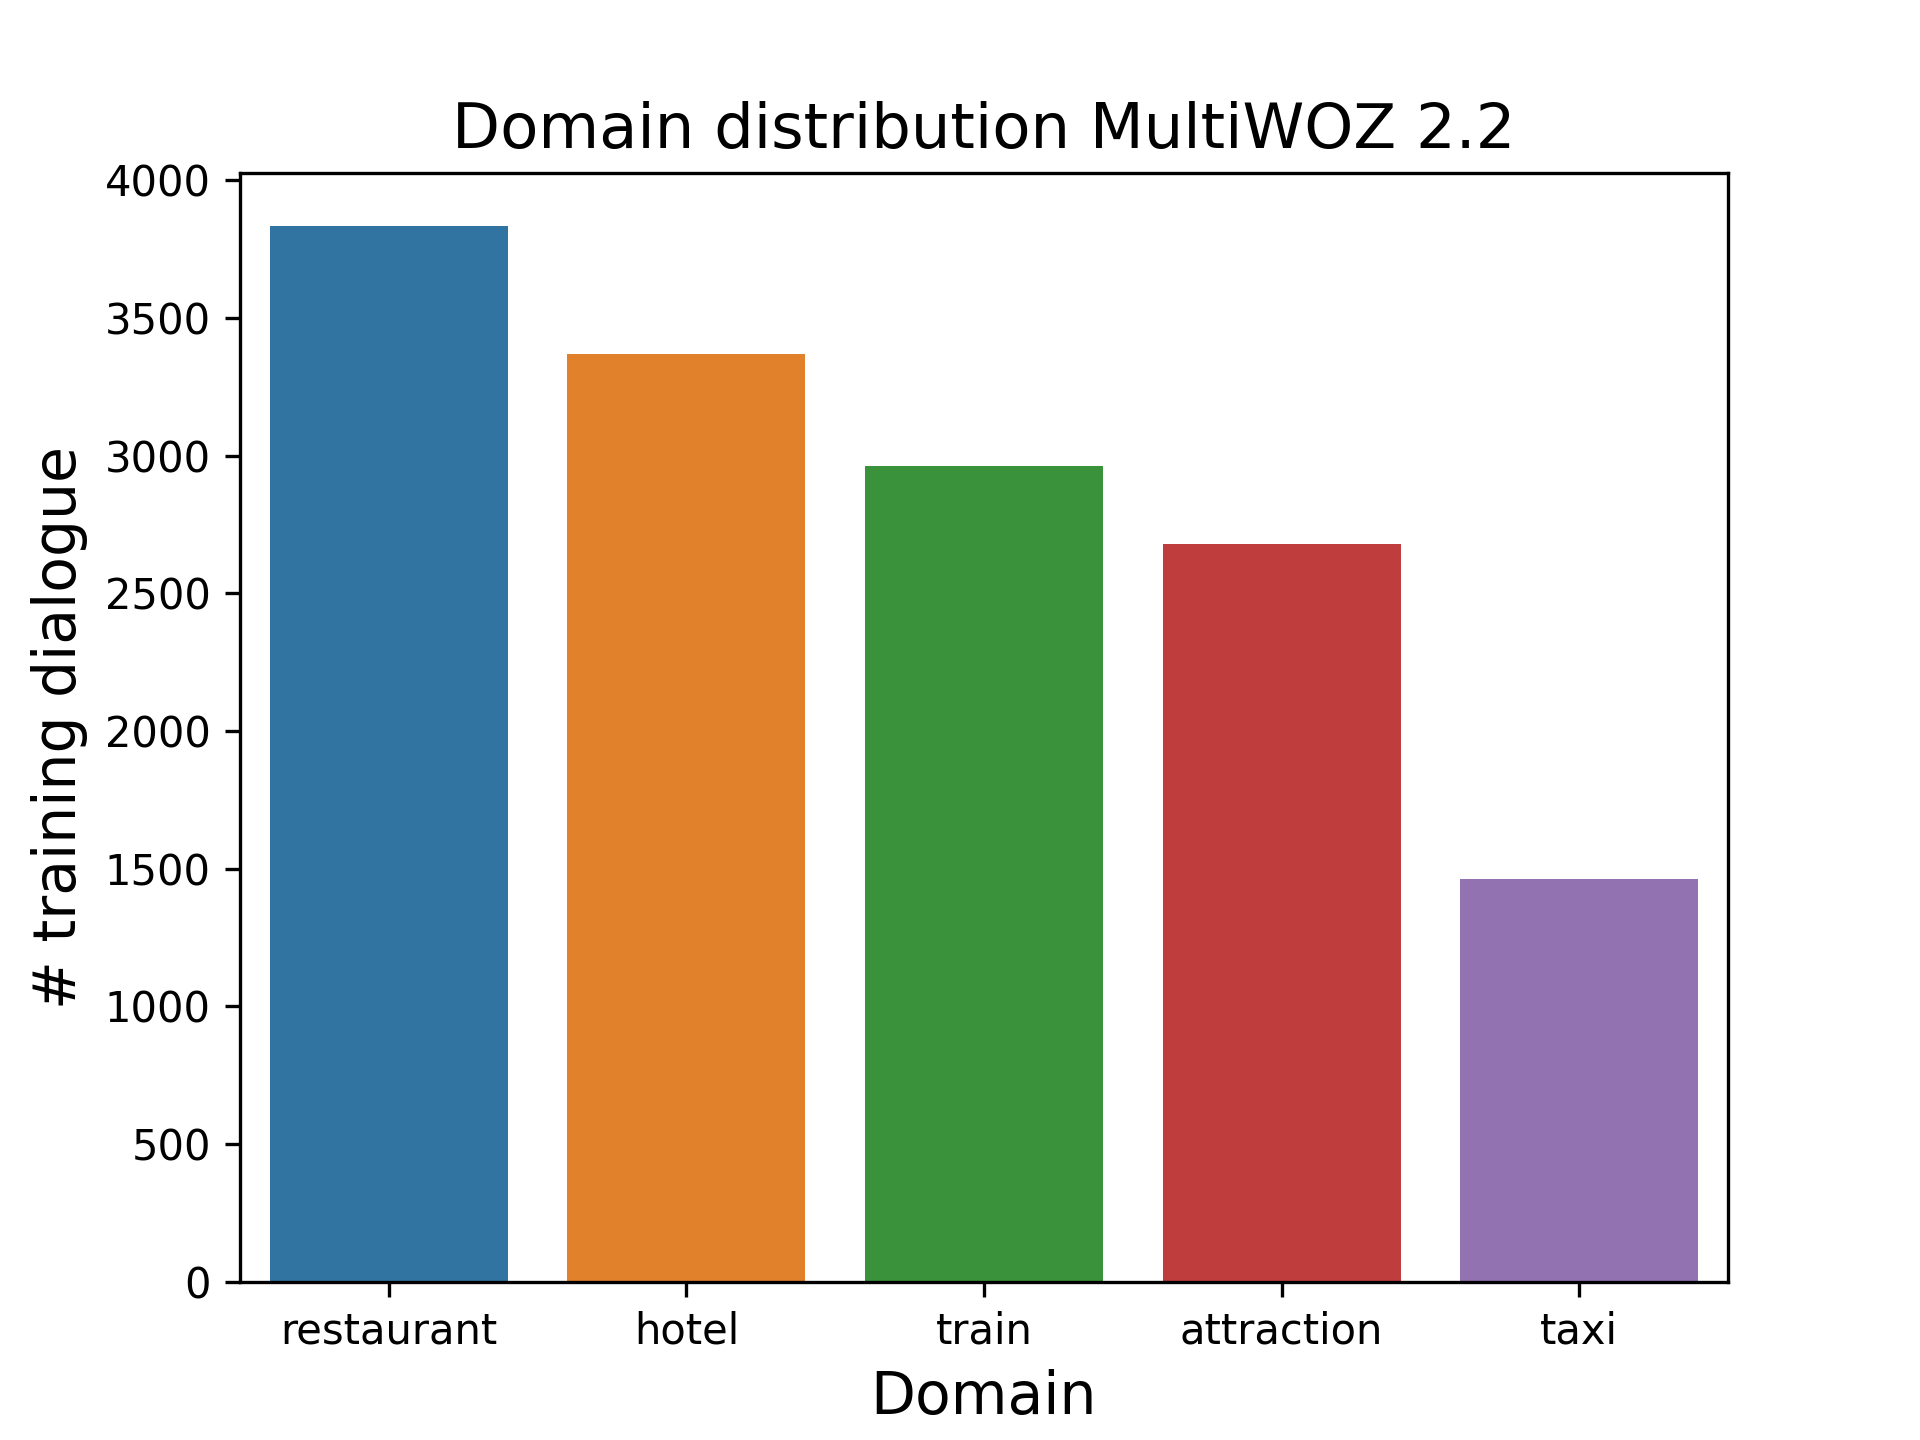
\includegraphics[width=0.8\textwidth]{images/multiwoz-distribution.png}
    \caption{The distribution of respective domains in the MultiWOZ dialogue dataset, showing how many of the dialogues contain the respective domain.}
    \label{02:fig:mw-dist}
\end{figure}


\section{Evaluation metrics}
\label
{02:sec:eval_metrics}
Here, we provide a set of commonly used metrics to evaluate the quality of dialogue modeling and response generation.
We also use some less common metrics for specific tasks.
Those metrics are described together with experiments in respective sections of this work.
\subsection{NLU metrics}
    \begin{itemize}
        \item \textbf{$F_1$ Score} (F-score, F-measure)~\cite{goutte2005probabilistic} is a widely used metric to evaluate binary classification.
    To measure F1 score, we first compute the number of occurrences of True Positives (TP), False Positives (FP), and False Negatives (FN).
    Subsequently we can compute Precision (P) and Recall (R) in the following way:
    \begin{equation*}
        P = \frac{TP}{TP + FP}; R = \frac{TP}{TP + FN}
    \end{equation*}
    The $F_1$ score is then computed as a harmonic mean of P and R:
    \begin{equation*}
        F_1 = \frac{2\cdot P \cdot R}{P + R}
    \end{equation*}
    $F_1$ score is sometimes used also to measure multiclass classification performance.
    Usually, two ways of $F_1$ generalization are used. \emph{Micro $F_1$ score} averages per-class $F_1$ scores with weights corresponding to the respective class frequencies whereas \emph{Macro $F_1$ score} considers all classes equally important.
    $F_1$ is a classification evaluation metric task, and in the context of dialogue NLU it is frequently used to evaluate the performance of slot filling.
        \item \textbf{Intent Accuracy} is the percentage of slot occurrences assigned into the correct intent cluster under the reference mapping.
        \item \textbf{Domain Detection Accuracy} is simply the ratio of cases in which the system correctly detects the domain.
        \item \textbf{Entity Match Rate (EMR)}~\cite{wen2016network} calculates the last turn's entity in each dialogue. Using the final constraints, it verifies if a correct entity would be retrieved from the database.
    \end{itemize}
\subsection{State tracking metrics}
    \begin{itemize}
    \item \textbf{Joint Goal Accuracy (JGA)}~\cite{mrkvsic2016neural} is computed as the ratio of dialogue turns for which the predicted belief state matches the ground truth.
    We use fuzzy matching of the slot values so that capitalization or minor typos do not influence the result.
    \item $F_1$ score on the slot level can also be used to evaluate the performance of state tracking
    \end{itemize}
\subsection{Dialogue-level metrics}
    \begin{itemize}
        \item The main \emph{overall measure} for evaluating a task-oriented dialogue is the dialogue \textbf{success rate} \cite{deriu_survey_2021}.
For MultiWOZ, we use the standard evaluation of dialogue success as the ratio of dialogues where the user reaches the desired goal, based on goal annotation provided with the data \cite{nekvinda-dusek-2021-shades}. 
The SGD dataset does not include goal annotation but contains information about the requested slots. Therefore, we compute SGD success rate as the proportion of dialogues in which (1) the system captures all the informed slots correctly and (2) all the requested slots are provided.
For more details about the inform and request slots, we refer the reader to Section~\ref{02:sec:input-data-desc}
    \item  \textbf{BLEU score} \cite{papineni-etal-2002-bleu} is largely used to evaluate response generation in machine translation, summarization, and other tasks, including dialogue generation.
    Although it has some flaws \cite{callison-burch-etal-2006-evaluating} and was designed mainly for corpus-based evaluation, it is widely used so it is desirable to measure it for comparison with other works.
\end{itemize}

There are multiple different criteria for dialogue systems evaluation.
In the case of modular systems, the individual modules can be evaluated separately.
It is considerably harder to measure a system's overall performance.
The policy module's decision is difficult to evaluate without turn-level action annotations.
BLEU usage is controversial for dialogue systems since it often fails to capture the semantics of the utterance, which is perhaps more critical than in the translation task \cite{lowe2017towards}.
It is also common to measure \textbf{Dialogue success rate}.
However, it is not straightforward how to define dialogue success robustly.
Many systems use user simulators to allow the employment of reinforcement learning techniques.
In such scenarios, the user behavior is model-based and can be non-deterministic. Therefore, defining success is challenging.
Usually, it is based on evaluating user and system dialogue acts, which relies on good and extensive data annotation.

\subsection{Human Evaluation}
Due to the mentioned challenges, \textbf{human evaluation} remains the best way to evaluate dialogue systems.
Human evaluation plays a crucial role in developing and refining dialogue systems. This is because automated tools or metrics often fail to capture the nuanced responses and language variations inherent in human communication. 

Dialogue systems, including chatbots and virtual assistants, are directly designed for human interaction, making their performances depend heavily on how effectively they can understand and respond.
Therefore, assessing their capabilities requires a human-like understanding of the conversations.

Moreover, human evaluation is important to measure aspects that go beyond the correctness of the system's responses. For instance, the engagingness of the conversation or the appropriateness of the system's tone requires human judgment. Also, human evaluators can better identify and evaluate cultural and social aspects than automated methods.

While human evaluations are more time-intensive and costlier than automated ones, they offer a more detailed, insightful, and accurate assessment of the dialogue system's performance.
Therefore, they are crucial for improving these systems to make them more user-friendly and effective for human interaction.